\documentclass{sig-alternate}
\usepackage{txfonts}
\usepackage{ifpdf}
\usepackage{amsmath}
\usepackage{mathrsfs}
\usepackage{amsfonts}
\usepackage{subfigure}
\usepackage{graphicx}
\usepackage{latexsym}
\usepackage{multirow}
\usepackage{microtype}
\usepackage{algorithm}
\usepackage{paralist}
\usepackage[sort]{cite}
\usepackage[pdfborder={0 0 0},plainpages,pdfpagelabels=false]{hyperref}

\setlength{\paperheight}{11in}
\setlength{\paperwidth}{8.5in}

\newtheorem{theorem}{Theorem}
\newtheorem{proposition}[theorem]{Proposition}
\newtheorem{claim}[theorem]{Claim}
\newtheorem{lem}[theorem]{Lemma}
\newtheorem{terminology}[theorem]{Terminology}
\newtheorem{corollary}[theorem]{Corollary}
\newtheorem{observation}[theorem]{Observation}
\newtheorem{problem}[theorem]{Problem}


\newtheorem{defi}[theorem]{Definition}
\newtheorem{exa}[theorem]{Example}

% QED symbol at the end of definitions and examples
\newif\ifqedwritten
\newenvironment{definition}[1][]{\begin{defi}[#1]\upshape\qedwrittenfalse}{\qedhere\end{defi}}
\newenvironment{example}{\begin{exa}\upshape\qedwrittenfalse}{\qedhere\end{exa}}
\newcommand{\qedhere}{\ifqedwritten\else\ifmmode\tag*{\qed}\else\hfill\qed\fi\global\qedwrittentrue\fi}

\newcommand{\topk}{\mbox{top-$k$}}
\newcommand{\Topk}{\mbox{Top-$k$}}
\newcommand{\topkm}{\mbox{top-$k$,$m$}}
\newcommand{\Topkm}{\mbox{Top-$k$,$m$}}

\renewcommand{\leq}{\leqslant}
\renewcommand{\geq}{\geqslant}

% More tolerant setting for floats -- more compactness
\renewcommand\floatpagefraction{.9}
\renewcommand\topfraction{.9}
\renewcommand\bottomfraction{.9}
\renewcommand\textfraction{.1}
\setcounter{totalnumber}{50}
\setcounter{topnumber}{50}
\setcounter{bottomnumber}{50}

\renewcommand{\textfloatsep}{1em}
\renewcommand{\dbltextfloatsep}{1em}

%%%%%%%%%%%%%%%  Magic for tighter spacing around theorem-like environments
\makeatletter
\def\@begintheorem#1#2{%
    \vspace{-3pt}
    \parskip -1pt
    \trivlist
    \item[%
        \hskip 10\p@
        \hskip \labelsep
        {{\sc #1}\hskip 5\p@\relax#2.}%
    ]
    \it
}
\let\old@endtheorem\@endtheorem
\def\@endtheorem{\old@endtheorem\vspace{-8pt}}
\makeatother

\begin{document}

%\conferenceinfo{SIGMOD '12,} {May 20--24, 2012, Scottsdale, Arizona, USA.}
%\CopyrightYear{2012}
%\crdata{978-1-4503-1247-9/12/05}
%\clubpenalty=10000
%\widowpenalty = 10000


\title{Exact and Approximate String Joins with Taxonomy}

%\numberofauthors{5}

\author{
%\alignauthor{Jiaheng Lu  \\
%       \affaddr{$^{\dag}$ School of Information and DEKE, MOE, Renmin
%University of China; Beijing, China}\\
%       \email{\{jiahenglu\}@ruc.edu.cn,  pierre@senellart.com}
%}
}


%For example, in XML keyword query refinement, each
%keyword is associated with a set of alternative terms.  Each term is
%associated with an inverted list containing the occurrences and the
%weights of the corresponding elements in the XML database. The
%\topkm{} queries return top-$k$ refined keyword combinations
%according to the corresponding \mbox{top-$m$} search results of keyword
%queries. In general, \topkm{} queries are useful in scenarios
%where the problem of selecting \emph{combinations
%of attributes} associated with ranked inverted lists naturally occurs.
%Applications range


\maketitle

\begin{abstract}

A string join finds all string pairs between two input string collections. It is an essential operation in
many applications, such as data integration and data cleansing. This paper investigates a novel challenge to integrate taxonomy into string joins. In general, the taxonomy presents a general-purpose strategy to improve the accuracy of string joins by enriching data with semantics-based knowledge  (i.e., a set of IS-A hierarchies). For example,  ``\textsf{California}'' is a state of ``\textsf{U.S.}'' in a geographical taxonomy.

In this work, we study both exact-join and approximate-join cases with taxonomy. Exact joins mean that two strings have the exact IS-A relation, while approximate joins extend the existing similarity functions to capture the IS-A relations against part of strings. Although approximate string joins were studied without taxonomy, we encounter new  challenges here: two strings, which are similar with a taxonomy-based similarity function, may not share any common token. That means, the existing signature-based filtering strategy do not work any more.  In this paper, we propose a set of novel algorithms and filtering strategies for both exact-joins and approximate-joins. The technique relies on the insight that two strings are similar only if they share certain number of common tokens and/or they have IS-A relations in the taxonomy.  The extensive performance evaluation shows that our algorithms can utilize the taxonomy to improve the effectiveness of string joins  and  scale very well with important parameters like data size and taxonomy size.


\end{abstract}

%\category{H.2.4}{Database Management}{Systems}[Query processing]
%\category{H.3.3}{Database Management}{Information Search and
%Retrieval}[Search process]

%\terms{Algorithms, Experimentation, Performance, Theory}

%\keywords{keyword search, package search, top-$k$ querying}

\section{Introduction}


\begin{figure}[t]
\centering
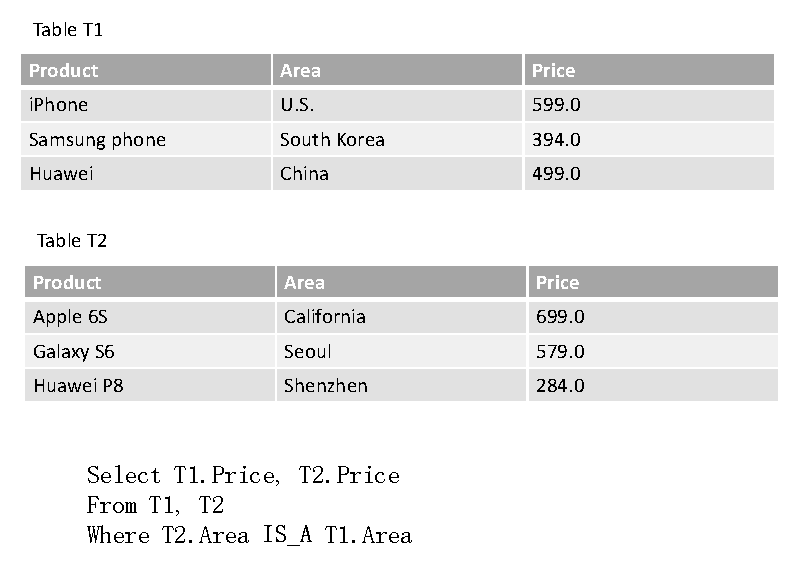
\includegraphics[width=0.45\textwidth]{figures/productexample}
 \caption{Examples to illustrate approximate joins}
\label{fig:autocompletion}
\end{figure}


\begin{figure}[t]
\centering
\includegraphics[width=0.45\textwidth]{figures/taxonomylabels}
 \caption{An example of taxonomy with labels}
\label{fig:taxonomy}
\end{figure}


Strings form a fundamental data type in computer systems and  string joins find all string pairs between two input string collections.  String joins are essential operations in
many applications, such as  data integration \cite{conf/sigmod/Sarawagi04}, data cleansing \cite{conf/vldb/ArasuGK06,journals/www/LiJM06} and data exploration. Conceptually, there are two types of string joins: exact joins and approximate joins. Exact joins mean that two matching strings should be exactly the same, while approximate joins tolerate certain difference
  between two strings and the similarity of two strings can be measured by a similarity function, such as  $n$-gram similarity~\cite{conf/spire/Kondrak05}, Levenshtein Distance
\cite{journals/pvldb/XiaoWL08,conf/sigmod/WangLF12}, Jaro-Winkler
measure~\cite{Winkler99thestate}, Jaccard
similarity~\cite{conf/icde/ChaudhuriGK06}, cosine
similarity~\cite{journals/ipm/SaltonB88}.


 Taxonomies are sets of IS-A hierarchies, which identify the relations between different concepts. For example, Figure \ref{fig:taxonomy} shows an example of taxonomy for geographical concepts. However, to the best of our knowledge, the integration of taxonomy information in data used for classifier training has never been investigated so far.




Given two strings, $s_1$ and $s_2$, we return three possible relationships between $s_1$ and $s_2$: hypernym, hyponym, mixed. For example, ``California, U.S.'' is a hyponym of ``U.S.'', ``Egypt'' is the same as ``Egypt, Africa Northern'' and ``Egypt'' is a hypernym of ``Africa''. For more examples: ``Egypt, Algeria'' is a hyponym of ``Africa Northern''.

There are two related problems: string join with taxonomy and string similarity join with taxonomy

The leave behind two intriguing questions:

1. How to efficient process string joins with taxonomy? And for multiple joins.


2. How to process the similarity joins and multiple-way similarity joins?  This question becomes increasingly urgent nowadays with the arrival of big data.

%\begin{problem}(String measure with taxonomy). Given two strings $s_1$ and $s_2$ and a taxonomy $T$, how to measure the similarity between $s_1$ and $s_2$ based on T?
%\end{problem}
%\begin{problem}(String joins with taxonomy). Given a string $p$$\in$
%$\Sigma^*$, an integer k, and a synonym set $\mathbb{R}$,  .
%\end{problem}




\subsection{Novelty and contributions}


\smallskip


Our contributions are as follows.

\noindent \textbf{Introduction of string joins with taxonomy}. We introduce a new problem to utilize the taxonomy for the string joins in databases, which has application in data integration and data cleansing.

\noindent \textbf{Optimal algorithms for string joins} We introduce a holistic algorithm for multiple string joins.

\noindent \textbf{Introduction of approximate string joins with taxonomy}: Provide three relationships Hyper, Hypo and mixed similarity.

\noindent \textbf{Novel algorithms for approximate string joins}


Finally, we perform experiments to evaluate our results and show the benefits of proposal algorithms.


\smallskip

The rest of this paper is organized as follows. Section 2
provides the necessary definitions, formulates . Section
3 includes our algorithm for exact joins with taxonomy. In Section 4, we study
the approximate string join, proposing our solution, analyzing its approximation
ratio, and presenting our similarity join algorithms.
Our experiments are presented in Section 5. Finally,
Section 6 concludes with a discussion about future work.



\section{Preliminaries} \label{sec:preliminaries}



In this section, we first  define taxonomy, including
hypernym and hyponym. Subsequently,
we discuss challenges of processing taxonomy-based approximate string joins.


\subsection{Taxonomy}

A taxonomy (T ,$\sqsubset$ ) consists of a universe of terms T and
a term-term hypernym-hyponym relationship $\sqsubset$.

Hypernym-hyponym relationship. The hypernym-hyponym relationship
$\sqsubset$ is a partial order T . For two terms t1 and t2,
we write t1 $\sqsubset$ t2 or t2 $\sqsubset$ t1, if t1 is a hypernym of t2 (or t2
is a hyponym of t1). For example, ``Caribbean Region'' is a hyponym of
``Americas''. Figure  \ref{fig:taxonomy} shows an example of taxonomy for geological locations.



Hyponymy shows the relationship between the more general terms (hypernyms) and the more specific instances of it (hyponyms). A hyponym is a word or phrase whose semantic field is more specific than its hypernym. The semantic field of a hypernym, also known as a superordinate, is broader than that of a hyponym. An approach to the relationship between hyponyms and hypernyms is to view a hypernym as consisting of hyponyms. This, however, becomes more difficult with abstract words such as imagine, understand and knowledge. While hyponyms are typically used to refer to nouns, it can also be used on other parts of speech. Like nouns, hyponyms in verbs are words that refer to a broad category of actions. For example, verbs such as stare, gaze, view and peer can also be considered hyponyms of the verb look.
Hypernyms and hyponyms are asymmetric. Hyponymy can be tested by substituting X and Y in the sentence ``X is a kind of Y'' and determining if it makes sense.[4] For example, ``A screwdriver is a kind of tool''  makes sense but not ``A tool is a kind of screwdriver''.


Hyponymy is a transitive relation, if X is a hyponym of Y, and Y is a hyponym of Z, then X is a hyponym of Z.[5] For example, violet is a hyponym of purple and purple is a hyponym of color; therefore violet is a hyponym of color. In addition, it should be noted that a word can be both a hypernym and a hyponym: for example purple is a hyponym of colour but itself is a hypernym of the broad spectrum of shades of purple between the range of crimson and violet.

The hierarchical structure of semantic fields can be mostly seen in hyponymy. They could be observed from top to bottom, where the higher level is more general and the lower level is more specific. For example, living things will be the highest level followed by plants and animals, and the lowest level may comprise dog, cat and wolf.

Under the relations of hyponymy and incompatibility, taxonomic hierarchical structures too can be formed. It consists of two relations; the first one being exemplified in 'An X is a Y' (simple hyponymy) while the second relation is 'An X is a kind/type of Y'. The second relation is said to be more discriminating and can be classified more specifically under the concept of taxonomy.

Computer science often terms this relationship an ``is-a'' relationship. For example, the phrase ``Red is-a colour'' can be used to describe the hyponymic relationship between red and colour.

Hyponymy is the most frequently encoded relation among synsets used in lexical databases such as WordNet. These semantic relations can also be used to compare semantic similarity by judging the distance between two synsets and to analyse Anaphora.

As a hypernym can be understood as a more general word than its hyponym, the relation is used in semantic compression by generalization to reduce a level of specialization.

%\begin{figure}[t]
%\centering
%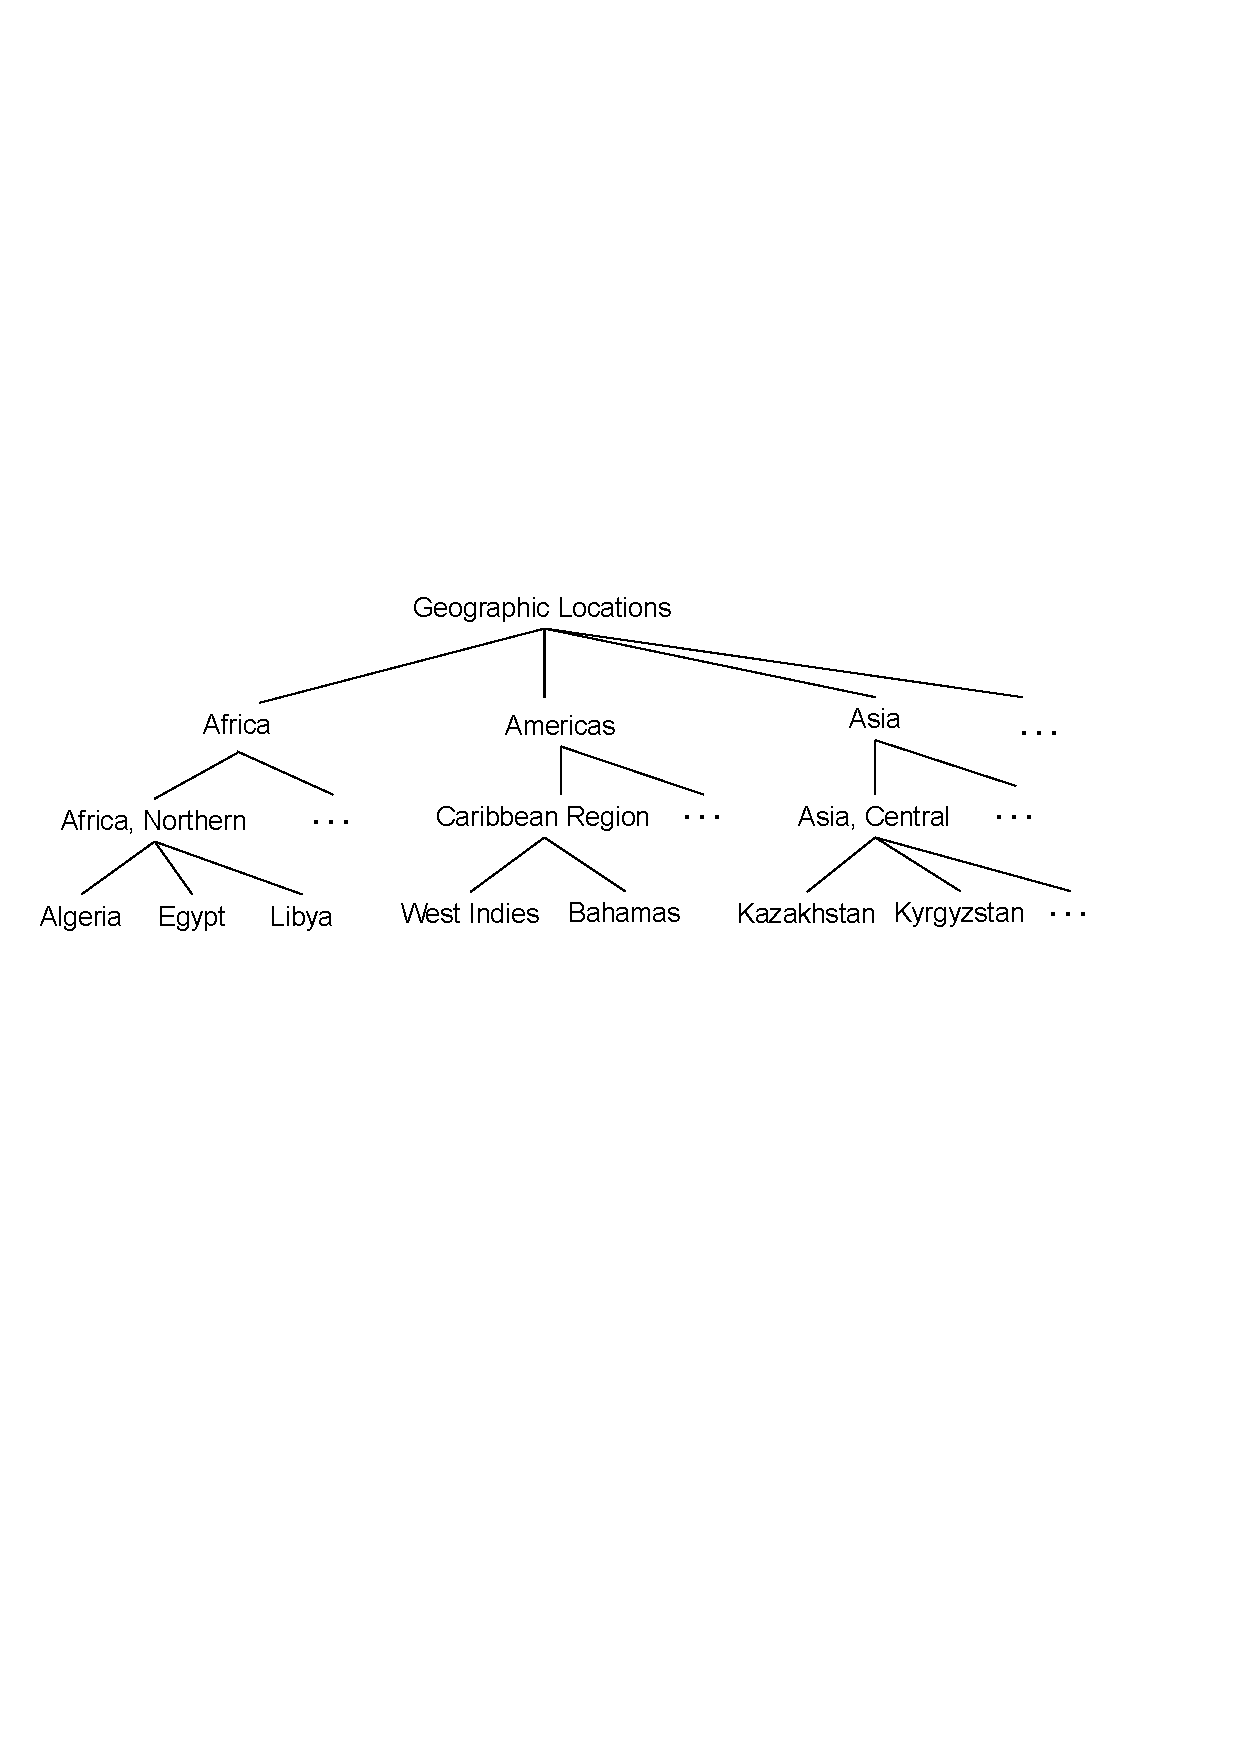
\includegraphics[width=0.45\textwidth]{figures/taxonomy}
% \caption{An example of taxonomy on ``\textsf{Geographic locations}''}
%\label{fig:taxonomy}
%\end{figure}

Example extended SQL

Select  T1.price, T2.price \\
From Table T1 and T2 \\
Where T1.area is\_a\_hypernym T2.area \\
With taxonomy T \\


The second SQL query:

Select  T1.price, T2.price, T3.price \\
From Table T1, T2, T3 \\
Where T1.area is\_a\_hypernym T2.area AND T1.product is\_a\_hypernym T2.product



\section{Taxonomy based joins for single match}
\label{sec:taxo_similarity}

In this section, we investigate a special case when a string matches only one node in a taxonomy tree, which will form a foundation to a generalised case studied in the next section.

\subsection{Similarity functions}

Given a taxonomy tree, we borrow an existing labelling scheme called \textit{Dewey code}, which is a prefix-based scheme that records the position of each node, according to the path from the root to the node. The IS-A relations between tree nodes can be determined easily. For example, Figure \ref{fig:toytaxonomyexample} shows an example of a taxonomy tree with Dewey codes. ``\textsf{California} (2.1.1.1)'' IS-A part of ``\textsf{U.S.} (2.1)'', because ``2.1'' is the prefix of ``2.1.1.1''. Based on the Dewey code, we can define the similaity between two nodes in a taxonomy tree as follows.



Given two nodes $n_1$ and $n_2$ labeled with Dewey codes on a taxonomy tree, the taxonomy similarity (TS) between $n_1$ and $n_2$,

\begin{equation}
 TS_{max}(n_1,n_2) = \frac{|LCP(n_1,n_2)|}{max(|n_1|,|n_2|)}
\end{equation}

\smallskip
\smallskip


One of the most popular edge counting measure is that proposed by Wu and Palmer \cite{conf/acl/WuP94} as follows:

\begin{equation}
TS_{sum}(n_1,n_2) = \frac{2|LCP(n_1,n_2)|}{|n_1|+|n_2|}
\end{equation}

The measure based on information content have a similar structure but instead of using the depth in the taxonomy they use an estimation of the information carried by the concpet. Different measures are characterized by different ways of estimating the information content, using either a data corpus or the intrinsic structure of the taxonomy.  A method which uses only the taxonomy structure has been proposed in \cite{journals/kbs/SanchezBI11}  where the information content of a concpet is expressed as the ratio between a measure of its generality (relatd to the number of ancestors) and a measure of its concreteness (related to the number of descendants). The specfic estimation of the information conetnt is described in Eq.



\begin{equation}
TS_{IC}(n_1,n_2) = \frac{2IC(LCP(n_1,n_2))}{IC(n_1)|+IC(n_2)}
\end{equation}


\begin{equation}
IC(n) = -log (\frac{|Leaves(n)|/|Ancestors(n)|+1}{|All~leaves|+1})
\end{equation}

\begin{example}
Consider Figure \ref{fig:toytaxonomyexample}, the similarity between ``\textsf{Seoul}'' (3.1.1.1) and ``\textsf{Suwon}'' (3.1.1.2) is $\frac{3}{4}$= 0.75 (as both countries locate in the same country: South Korea.), but the similarity between ``\textsf{Seoul}''  (3.1.1.1) and ``\textsf{Shenzhen}'' (3.2.1.1) is only $\frac{1}{4}$= 0.25 (as two countries locate in the different countries, but the same continent: Asia).
\end{example}


% In the worst case, the time complexity to compute the taxonomy similarity is linear to the length of the Dewey codes of nodes $n_1$ and $n_2$. 


\subsection{Join algorithms for sorted lists}

Given two collections of strings $S_1$ and $S_2$,  a \textit{similarity join} finds all pairs $(n_1, n_2) \in S_1 \times S_2$,
such that $TS(n_1,n_2)$ $>$ $\theta$, where $\theta$ is a predefined threshold. A baseline algorithm is the nested-loop join, which generates all string pairs to verify their similarities.  Obviously, this baseline involves many unnecessary verifications for string pairs which cannot contribute to final answers. We next propose two families of algorithms to speed up the processing.

\begin{algorithm}
{\bf Input}: two sorted lists  $L_1$ and $L_2$\\
{\bf Output}: pairs $R$ =\{$(s_1,s_2) \in L_1 \times L_2$ | $TS(s_1, s_2) > \theta$\}
\begin{compactenum}[(1)]
\item {\bf FOR}  i =1 and 2 {\bf DO}
\item ~~ Initialize two pointers $C_i^1$ and $C_i^2$ to the first element of  $L_i$
\item {\bf WHILE}  ($\neg$end($L_1$) and $\neg$end($L_2$)) {\bf DO}
\item ~~ $min$ = $\arg\min_{i}$($cur(C_i^1)$); $max$ = $\arg\max_{i}$($cur(C_i^1)$)
\item ~~ Let $p$ denotes the prefix of $cur(C_{min}^1)$ with the length $  \lceil l \cdot \theta \rceil$
\item ~~ $C_{max}^2$ =$C_{max}^1$
\item ~~ {\bf WHILE} ($p$ is a prefix of (cur($C_{max}^2$) ) {\bf DO}
\item ~~ ~~ ~~ {\bf IF} TS(cur($C_{max}^2$), cur($C_{min}^1$))$> \theta$ {\bf THEN}
\item ~~~   ~~ ~~ ~~ Add (cur($C_{max}^2$), cur($C_{min}^1$)) to $R$
\item ~~ ~~ ~~ advance($C_{max}^2$)
\item ~~   advance($C_{min}^1$)
\item  {\bf Return} $R$
\end{compactenum}
\caption{TS Join based on sorted labels}
\label{alg:exactjoin}
\end{algorithm}





The first optimization is to sort the lists in advance. Given a collection of strings $S$,  a list $L_S$ contains the \textit{Dewey} codes of the taxonomy tree nodes that match strings. The labels in the list are sorted by the ascending lexicographical order. The operations over lists are: \textit{advance} and \textit{end}, which move the cursor of a list to the next position and test if the cursor points to the end of a list, respectively.



Algorithm \ref{alg:exactjoin} shows the pseudo-code of a string join based on sorted lists. There are two cursors $C_1$ and $C_2$ in each list. This algorithm repeatedly finds the pairs that share the certain number of common prefixes, by iterating though the list in sorted order, and return the answers. In particular,  for each accessed node $n$ pointed by the cursor $C^1_{min}$, the algorithm read all nodes  which share the certain number of the common prefix with $n$, i.e. $ \lceil |n| \dot \theta \rceil$, which are pointed by the cursor $C^2_{max}$ and calculate the similarity between two string to find all results. In Line 5, $l$ is the length of  $cur(C^1_{min})$.

\begin{example} See Figure \ref{fig:sortJoin}(a). We use this example to illustrate Algorithm \ref{alg:exactjoin}. The join threshold is 0.6. First the two points $C_1$ and $C_2$ point to the first elements. Note that there is no LCP computation from 1.1 to 1.4. Then pointers go forward to find the pair $(1.5.4, 1.5.5.1)$. Their similarity is less than 0.6, but 2/3 $>$ 0.6. So the pointers need to visit 1.5.5.1 to 1.5.5.4. Then finally, the algorithm find the matched pairs 1.5.5 and 1.5.5.1 to 1.5.5.4.  
\end{example}

The following lemma is a key to establish the correctness of Algorithm \ref{alg:exactjoin}. The proofs and Lemma and Theorem can be found in Appendix.

\begin{lem} Given a string $s$ with the length $|s|$, if any string t, $TS(s,t) > \theta$,  then $s$ and $t$ share the prefix with the length of at least $|s| \cdot \theta $.
\label{lemma:sortjoinlength}
\end{lem}

\begin{theorem} Algorithm \ref{alg:exactjoin} correctly finds all results for the string joins. In the worst case, the time complexity is  $O(|L_1| \cdot |L_2| \cdot n)$, where $n$ is the length of the longest string. \label{theo:sortedjoin}, $|L_1|$ and $|L_2|$ denote the cardinality of two lists.
\end{theorem}




\begin{algorithm}
{\bf Input}: two sorted lists  $L_1$ and $L_2$\\
{\bf Output}: pairs $R$ =\{$(s_1,s_2) \in L_1 \times L_2$ | $TS(s_1, s_2) > \theta$\}
\begin{compactenum}[(1)]
\item {\bf FOR}  i =1 and 2 {\bf DO}
\item ~~ Initialize two pointers $C_i^1$ and $C_i^2$ to the first element of  $L_i$
\item Let $x$ = $|LCP(cur(C_1^1),cur(C_2^1))|$
\item $min$ = $\arg\min_{i}$($cur(C_i^1)$); $max$ = $\arg\max_{i}$($cur(C_i^1)$)
\item {\bf WHILE}  ($\neg$end($L_1$) and $\neg$end($L_2$)) {\bf DO}
\item ~~ $C_{max}^2$ =$C_{max}^1$
\item ~~ $y = x$
\item ~~ {\bf WHILE} ($y \geq \lceil |cur(C_{min}^1)| \cdot \theta  \rceil$) {\bf DO}
\item ~~ ~~ ~~ {\bf IF} ($\frac{y}{max(|cur(C_{max}^2)|,|cur(C_{min}^1)|)}$ $> \theta$) {\bf THEN}
\item ~~ ~~ ~~ ~~ ~~ ~~ Add  the pair ($cur(C_{max}^2),cur(C_{min}^1)$) to $R$
\item ~~ ~~ ~~  advance($C_{max}^2$)
\item ~~ ~~ ~~ {\bf IF} $y > LP(C_{max}^2)$  {\bf THEN} $y$ = $LP(C_{max}^2)$
\item ~~ advance($C_{min}^1$)
\item ~~  {\bf IF} $x > LP(C_{min}^1)$  {\bf THEN}
\item ~~ ~~ ~~ $x$ = $LP(C_{min}^1)$ and exchange the values of $min$ and $max$
\item ~~ ~~ {\bf ELSE IF}  $x == LP(C_{min}^1)$  {\bf THEN}
\item ~~ ~~~~ ~~~~ ~~ recompute $x$, $min$ and $max$ as Lines (3) and (4)
\item {\bf Return} R
\end{compactenum}
\caption{Optimized TS Join based on sorted labels}
\label{alg:LCPSortJoin}
\end{algorithm}


 Algorithm \ref{alg:exactjoin} needs to compare two strings frequently  in Lines 4,7 and 8. When the string is long, this may takes a lot of time. We next propose an optimization to speed up this processing.

 We employ an index called  $LP(n)$, which is the length of the LCP between the node n and its preceding node. See the node ``1.1.2'' in the list $L_1$ of Figure \ref{fig:sortJoin}. LP(1.1.1) = 2, since LCP(1.1.1,1.1.2)=2.  We now introduce an algorithm to reduce the number of string comparison in Algorithm 2. Similar to Algorithm \ref{alg:exactjoin}, we maintain two cursors C1 and C2 for each list. But the main difference between Algorithm 2 and Algorithm 1 is that we avoid the prefix checking to compute the LCP. Unlike Line 7 in Algorithm 1, Algorithm 2 do not compute LCP and compare the length of strings. We use the preprocessing LCP values and avoid the computation of LCP in most cases. Therefore, we achieve better performance.
 
 We now go through Algorithm \ref{alg:LCPSortJoin}. In Line 1 and 2, it initialize two pointers for each list. In line 3, x denotes the length of LCP of two current elements. Line 4 compute the current min and max element. In Line 5 to 17, it iteratively access all elements in two lists. Line 6, set two pointers in the max list to be equal. y is a variable to recode the the length of LCP for two elements in the  $cur(C_{max}^2$) and $cur(C_{min}^1)$. In Line 9 and 10, we do not need to compute LCP, but we can know the results. The correctness can be proved in Lemma. In Line 12, update the length of LCP, but we can directly derive from LP. In line 14 to 17, update the length of LCP for two current element pointed by  $cur(C_{i}^1)$. The correctness can be proved in Lemma .
 
 z is the necessary prefix to satisfy the similarity. In Line 8, if the length of the two elements satisfy the condition in Line 9, we do not need to compute the similarity, but directly add them to the result R. Line 11 consider the next element and update the LP (reduce it if necessary). Line 12 to 19 recompute the LCP to x. If $x <> LP(C_{min}^1)$, we can avoid the LCP computation. We can save the cost a lot in this step.  

%\begin{figure}[t]
%	\centering
%	\includegraphics[width=0.22\textwidth]{figures/joinExample}
%	\caption{Illustration to join algorithm}
%	\label{fig:join}
%\end{figure}
%
%\begin{figure}
%	\centering
%	\includegraphics[width=0.5\textwidth]{figures/figureExampleRef}
%	\caption{Illustration to join algorithm}
%	\label{fig:triejoin}
%\end{figure}
%
%\begin{figure}
%	\centering
%	\includegraphics[width=0.25\textwidth]{figures/trieExample}
%	\caption{Illustration to join algorithm}
%	\label{fig:triejoin}
%\end{figure}


\begin{figure}[t]
\centering
\includegraphics[width=0.5\textwidth]{figures/joinExample2}
 \caption{Illustration to the optimized sorted join algorithm. Each item is a binary tuple: (Dewey, LP). The join threshold $\theta >$ 0.6 }
\label{fig:sortJoin}
\end{figure}

\begin{example} We use this example to illustrate Algorithm \ref{alg:LCPSortJoin}. Compared to Algorithm 1. the main difference is that we can avoid the computation of LCP from 1.5.5.2 to 1.5.5.4, since we LP=3, we can advance it in Line 14. When the list is long, it can save more computation of LCP. 
\end{example}

The following lemma is a key to establish the correctness of Algorithm \ref{alg:LCPSortJoin}.

\begin{lem} Let A, B and C be three Dewey codes,

(a) If $LCP(A,B) \neq LCP(B,C)$,  then $LCP(A,C)$ = min\{$LCP(A,B)$, $LCP(B,C)$\}.

(b) If $A>B$, $C>B$ and $|LCP(A,B)|>|LCP(B,C)|$ , then $C>B$.
\label{lemma:LCPcomparison}
\end{lem}

\begin{theorem} Algorithm \ref{alg:LCPSortJoin} correctly finds all results for the string joins. \label{theorem:LCPSortCorrectness}
\end{theorem}


We can show that the worst time complexity is bounded by the product of the size of two collections plus with a sum of LCP array, which is defined as the LCP sum of alternative elements, which is better than Algorithm 1.



\begin{definition} [LCP Array] Given two sorted sets of Dewey codes $S_1$ and $S_2$, first merge and sort $S_1$ and $S_2$ to one list S=$S_1 \cup S_2$, and for an elment $i$ in S, is the length of the LCP with the previous one for the element i in S, denoted as $LCPA_i(S1,S2)$.
\end{definition}

\smallskip

\begin{theorem} The TS join based on LP perform the join for two tables $T_1$ and $T_2$ in the worst complexity is $\mathcal{O}$$(S+|T_1||T_2|)$, where S= $\Sigma LCP(e,e')$, $e$ and $e'$ are two adjacent labels from the different tables in the merged sorted list.
\end{theorem}

\smallskip

Algorithm \ref{alg:LCPSortJoin} improves Algorithm \ref{alg:exactjoin} by reducing the cost for prefix computations. Unfortunately, Algorithm \ref{alg:LCPSortJoin} is not guaranteed to be optimal, in that the computation cost is not bounded by the size of input and output data. See an example of sub-optimality as follow. Recall Figure \ref{fig:sortJoin}. There are no answers for 1.5.4, and the accesses from 1.5.5.1 to 1.5.5.4 are useless. Therefore, this is not an optimal algorithm. In the next section, we seek to overcome this sub-optimality using a compact trie.

\subsection{Join algorithms with compact tries}

 Trie is a rooted tree with the following properties: Edges are labelled with symbols from an alphabet $\Sigma$. For every node $v$, the edges from $v$ to its children have different labels. Each node represents the string obtained by concatenating the symbols on the path from the root to that node. Compact tries reduce the number of nodes by replacing branchless path segments with a single edge. There are two kinds of nodes in compact trie. One is the real number with rectangle. The other is the internal node, which add an integer to indicate the shortest real element under the subtree. The construction and maintenance of a TC-trie is very similar to those in a compact trie, using the prefix as the key; the difference is that the I values in the internal node need to be propagated up the index structure.

%\begin{figure}[t]
%\centering
%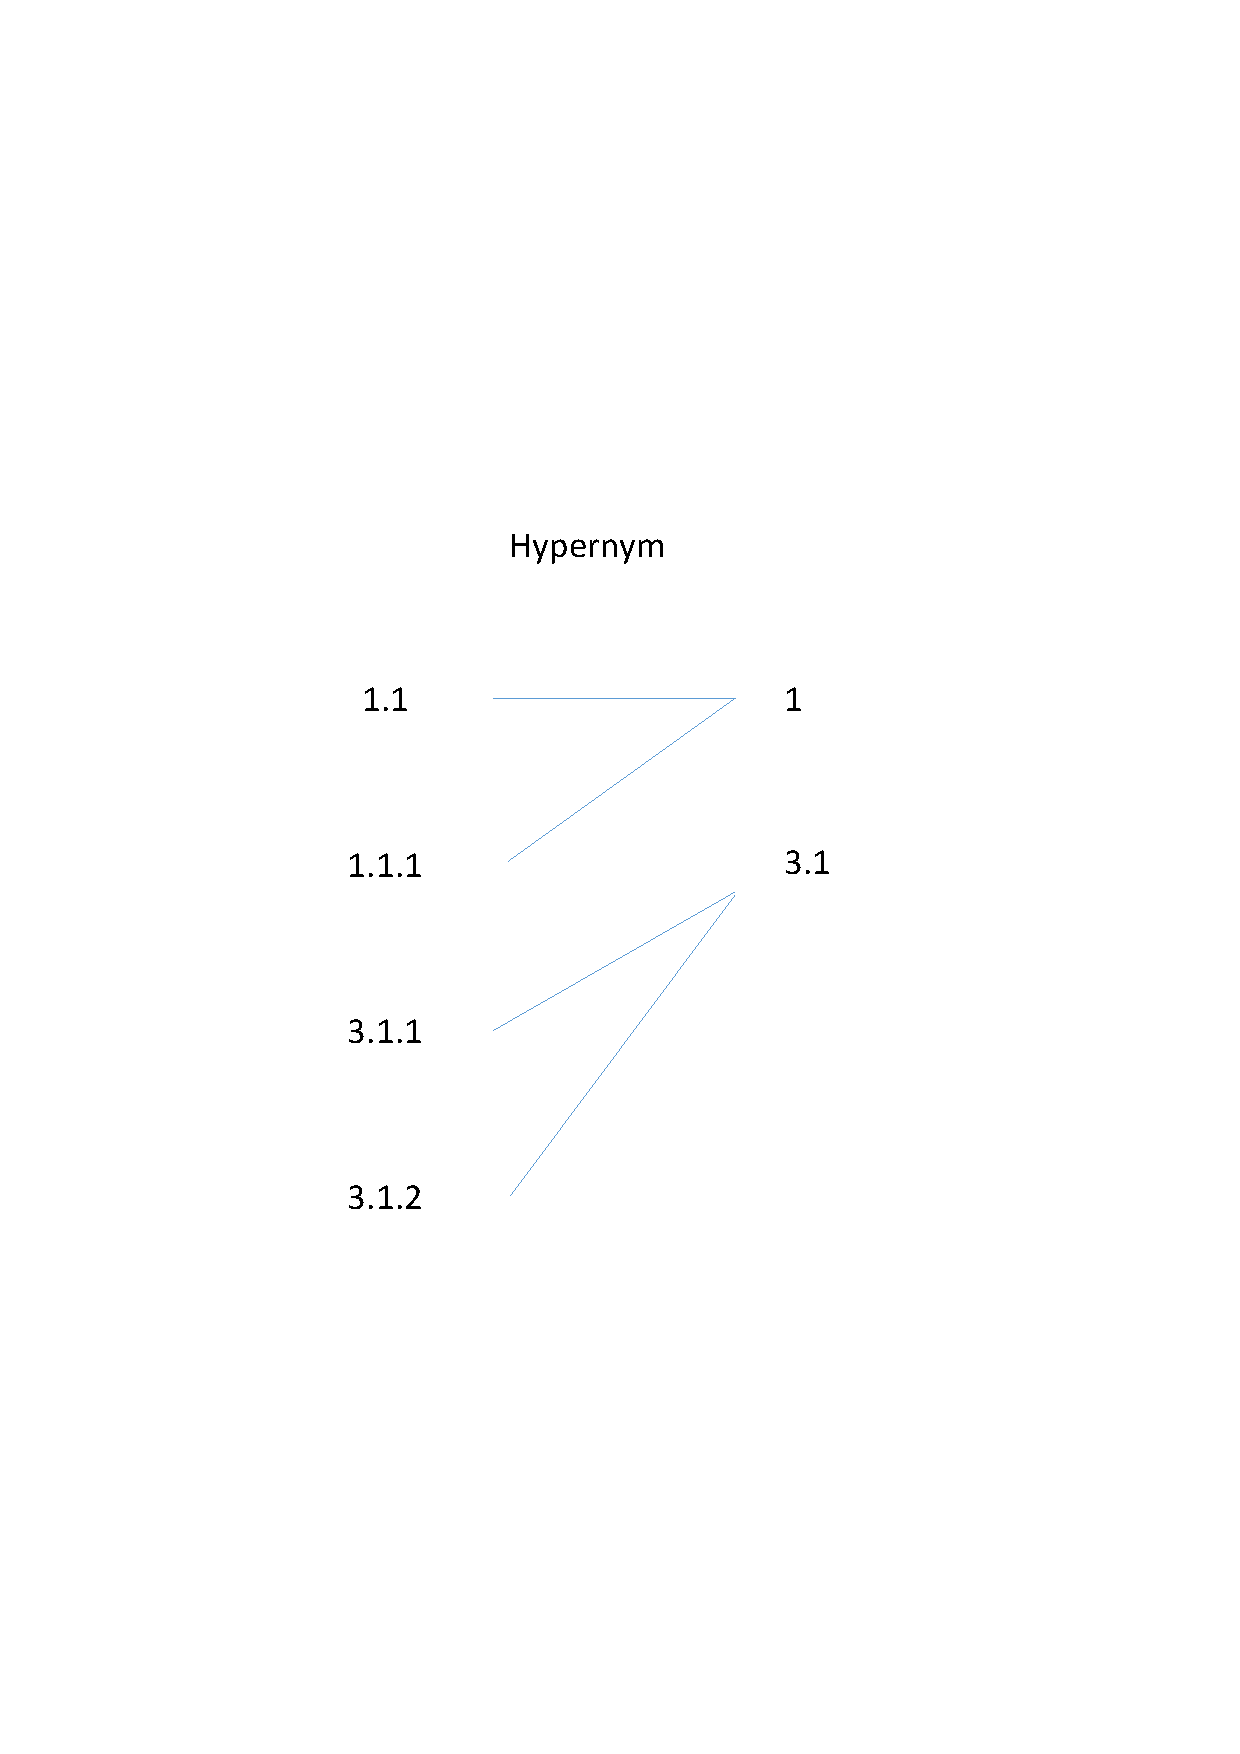
\includegraphics[scale=0.4]{figures/labeljoins}
% \caption{Join inverted lists}
%\label{fig:invertedlist}
%\end{figure}

%The worst case complexity is $O(N^2)$, because the algorithm may compute each pair of strings with the prefix $p$. But this algorithm will skip many pairs of string for comparison. A theoretical analysis based on a random string model show that the average complexity is $O(\frac{N^2}{S^{\lfloor (1-\theta) \cdot l \rfloor}})$, where $N$ is the total number of elements in each list and $S$ is the maximal width of the taxonomy.




%\begin{figure}[t]
%\centering
%\includegraphics[width=0.35\textwidth]{figures/prefixTrees}
% \caption{An example of TS join based on prefix trees (a circle means an internal element, but a rectangle means a real element)}
%\label{fig:taxonomyexample}
%\end{figure}



\begin{algorithm}
{\bf Input}: two collections of taxonomy nodes $S_1$ and $S_2$,  a threshold $\theta$ \\
{\bf Output}: string pairs $(s_1,s_2) \in S_1 \times S_2$, s.t. $TS(s_1, s_2) > \theta$
\begin{compactenum}[(1)]
\item Let $T_s$ and $T_t$ denote two compact tries for $S$ and $T$ respectively.
\item Initialize two cursors in two tries to point to the first real nodes
\item {\bf WHILE} ($\neg end(T_s) \wedge  \neg end(T_t)$) {\bf DO}
\item  ~~ $min$ = $\arg\min_{i}$($cur(C_i)$); $max$ = $\arg\max_{i}$($cur(C_i)$)
\item  ~~ {\bf IF} (possibleMatch(cur($T_{min}$),cur($T_{max}$))) {\bf THEN}
\item ~~ ~~ {\bf  IF} ($cur(T_{min})$ is an element)  {\bf THEN}
\item ~~ ~~  ~~ ~~ getResults(cur($T_{min})$,cur($T_{max}$))
\item ~~~~ advance($T_{min}$)
\item ~~ {\bf ELSE} Jump($T_{min}$)
\end{compactenum}
\smallskip
\textbf{Function} possibleMatch($s_1$,$s_2$)
\begin{compactenum}[(1)]
\item  $x =| LCP(s_1,s_2) |$
\item {\bf IF}  $x > \theta \cdot max (s_1, s_2 )$  {\bf THEN} RETURN TRUE
\item   ~~ {\bf ELSE} RETURN FALSE
\end{compactenum}
\smallskip
\textbf{Procedure} Jump($T$)
\begin{compactenum}[(1)]
%\item  read the next real node that is not a descendant of $cur(T)$ with the depth-first traversal
\item  find the smallest real node in T which share at least  $\theta cur( T_{max}$) 
\end{compactenum}
\smallskip
\textbf{Procedure} getResults($s_1$,$s_2$)
\begin{compactenum}[(1)]
\item  {\bf FOR EACH} ancestor $p$ (including $s_2$) of $s_2$ in  $T_{max}$ {\bf DO}
\item   ~~~ $x=LCP(p,s_1)$
\item   ~~~ {\bf FOR EACH} real nodes $s_i$ of the descendants of $p$  s.t.  $s_i > s_2$ and $|s_i| <= \lfloor |x|/ \theta \rfloor $ {\bf DO}
\item ~~~~~~~~ Add ($s_1,s_i$) to $R$;
\end{compactenum}
\caption{String joins with compact tries}
\label{alg:compactTrieJoin}
\end{algorithm}


We maintain a pointer $C$ to the node in TC trie. There are two operations over the TC-trie that affects this pointer:

1. \textsf{Advance} We advance $C$ to the next node in the trie with depth-first traversal.

2. \textsf{Jump} We jump $C$ to the right sibling node.

Initially $C$ points to the root node of TC trie. When C points to the last node in two TC tries and we advance it, we finish the traversal.

Algorithm \ref{alg:compactTrieJoin} shows the pseudo-code for string join with compact tries. The main idea is to use the trie to skip the nodes which cannot contribute to the final results. We  go through the algorithm. Line 5 determine if the current two elements can match. If yes, then we get results and then adance the minimal element. In line 7, we access the tree to find all element which can match $cur(C_{min})$. In Procedure getResults, we access the descendant of p only if there exists a node by minLen which is less than $ \lfloor |x|/ \theta \rfloor $.


\smallskip
\smallskip

\begin{example}
Consider the example in Figure \ref{fig:sortJoin}c, $\theta$=0.6. First, the cursors point to 2 and 2. possibleMatch return true. Compared to previous example, note that the accesses from 1.5.5.1 to 1.5.5.4 fro 1.5.4 are jumped. Therefore, it is optimal for this case.
\end{example}

\smallskip
\smallskip


\begin{theorem} Given two collections of nodes and a threshold $\theta$, Algorithm \ref{alg:compactTrieJoin} correctly finds all pair $n_1$ and $n_2$ such that $TS(n_1,n_2) > \theta$.
\end{theorem}

The correctness of the above theorem and the procedure of \textit{getResults} in the algorithm is based on the following lemma:

\begin{lem} Given two labels $s$ and $t$,  assume that $LCP(s,t) = x$. without the loss of generality, assume that $s<t$ by the lexicographical order, $TS(s,t) > \theta$ if and only if  $ x > \theta |s| $ and $  |t| < max(\frac{x}{\theta},|s|)$.
\end{lem}
\begin{proof}  $TS(s,t) > \theta$ $\Leftrightarrow$ $\frac{x}{|s|+|t|-x} > \theta \Leftrightarrow |t| < (\frac{1}{\theta}+1)x-|s|$. In addition, note that $|t| \geq x$. Then $x < (\frac{1}{\theta}+1)x-|s|$ $\Rightarrow$ $x > \theta |s| $, which concludes the proof.
\end{proof}


We next show the optimality: Given two compact tries, Algorithm \ref{alg:compactTrieJoin} takes each node and find the  matching node with the trie operations. Therefore, each accessed pair $C_1$ and $C_2$ belong to the final results. Since the operation of output Line is equal to the size of the final results: we have the following optimality result:

\begin{theorem}   The computing cost of Algorithm \ref{alg:compactTrieJoin} is linear to the sum of the size of the input and output. \label{theo:optimality_compactTrie}
\end{theorem}

\begin{proof}  The algorithm finds an answer in Procedure finds. Therefore, the optimality can be guaranteed.
\end{proof}





\section{String similarity joins with taxonomy}


We extend our definition to composite relation. For example: ''U.S and China'' is a composite hyponym of ``California and Beijing''. Another example: ``Hong Kong and California'' and ``U.S.''. This is a partial hypernym relation, since only California is a hypernym of U.S.

The sort-merge algorithm cannot work here.

Labeling scheme and the join:

If there are more than one string, then we can perform the verification after the filtering.


 Therefore, we propose a labeling scheme to process. Convert it to the ancestor-descendant joins



\subsection{Similarity measures}



We define the taxonomy similarity between two strings:

\begin{definition}[Taxonomy intersection]
Given two token sets $S_1$ and $S_2$, and a taxonomy $\mathcal{T}$, we say an element (token) $e \in S_1 \bigcap_T S_2$, if $ \exists E \subseteq S_1$ and $e \in E$, and $\exists T \subseteq S_2$, s.t. $\exists (E,T) \in \mathcal{T}$.\end{definition}


\noindent \textbf{Remark.}  Given two strings $s$ and $t$, it is clear that $|s \cap t| \leq min (|s|,|t|)$. But based on the taxonomy intersection, it is possible that $|s \cap_T t| > |s| $ or $|s \cap t| > |t| $. For example, s=``California'', t=``U.S.'', $|s \cap_T t|$ = 2.

\begin{definition}[Taxonomy-based Jaccard]   Given two sets of tokens $S_1$ and $S_2$,  the taxonomy-based Jaccard (TJ) between $S_1$ and $S_2$ is that:

\begin{equation}
TJ(S_1,S_2)=  \frac{(S_1 \bigcap_T S_2) \bigcup (S_1 \bigcap S_2) }{S_1 \bigcup S_2}
\end{equation} \end{definition}

\begin{algorithm}
{\bf Input}: two strings $s_1$ and $s_2$, a taxonomy $\mathcal{T}$ \\
{\bf Output}: $TJ(s_1,s_2,\mathcal{T})$
\begin{compactenum}[(1)]
\item Let $S_T $ to contain all tokens for taxonomy-based intersection. Initially, $S_T = \emptyset$.
\item Let $L_1$ (resp. $L_2$) denote the applicable taxonomy node list for $s_1$ (resp. $s_2$);
\item Scan $L_1$ and $L_2$ sequentially to find any matching pair $n_1 \in L_1$, $n_2 \in L_2$, s.t. ($n_1$,$n_2$) has the IS-A relation in $\mathcal{T}$;
\item Add all tokens $t \in n_1 \cup n_2$ to the set $S_T$;
\item  return $\frac{S_T \cup (|s_1 \cap s_2|)}{|s_1 \cup s_2|}$;
\end{compactenum}
\caption{String joins with taxonomy}
\label{alg:exactjoin}
\end{algorithm}

The time complexity of the TJ is $O(|s_1|+|s_2|+|n_1|+|n_2|)$, where $n_1$ (resp. $n_2$) denotes all applicable taxonomy nodes for string $s_1$  (resp. $n_2$). Assume that the preprocessing step finds the taxonomy relation for each string. Then the online algorithm only needs to find the matching IS-A relation between two strings to compute the intersection set with taxonomy.

\subsection{String similarity join algorithms}


%\begin{figure}[t]
%\centering
%\includegraphics[scale=0.4]{figures/tgsql2}
% \caption{Taxonomy graph example }
%\label{fig:similaritygeaph}
%\end{figure}



\textbf{Baseline algorithm}. We can use the similar algorithm as that in string exact join with taxonomy. And then use these candidate for filtering. But this baseline algorithm has one limitation that there are too many candidates. Then we show how to perform the second filtering to reduce the number of candidate pairs.

\textbf{Signature-based index}. Given a string s with length $|s|$, then the size of signature is $\lceil (1-\theta)|s| \rceil$. But if the signatures involve the taxonomy, then we cannot make this argument.

But if in some real cases, we select the word from taxonomy as signatures. Therefore we need to compute a relax maximum similarity. In this case, we still do not need to retrieve the whole string to compute real similarity.

Given as string $s$, assume that its applied taxonomy node is $n$.

In this paper, we propose a new index which combine a signature filters and a length together with a bit-matrix, which extends bloom filter to two dimensions.

In the literature, the current "modus operandi" is called \textit{prefix filter}, which is based on the intuition that if two canonicalized records are similar, some fragments of them should overlap with each other, as otherwise the two records
won't have enough overlap. This intuition can be formally captured by the prefix-filtering
principle \cite{conf/icde/ChaudhuriGK06} rephrased below.

\begin{lem} (\textsc{Prefix filter principle}) \cite{conf/icde/ChaudhuriGK06} Given an
ordering $O$ of the token universe $U$ and two strings $s$ and $t$, each with tokens sorted in the
order of $O$.   If Jaccard($s, t$) $\geq \theta$, then the first $\lceil(1-\theta)|s|\rceil$ smallest
tokens of $s$ and the first $\lceil(1-\theta)|t|\rceil$ smallest
tokens of $t$  must share at least one token.
\end{lem}

\subsubsection{N-ary prefix scheme}




Given a string $s$, we can construct the $n$-ary prefix token combination as follows:  Given an
ordering $O$ of the token universe $U$, we select $n$ tokens from the first $\lceil (1-
\theta) \cdot |s| \rceil + n -1$ in $s$. Then let $B^s_n$ denote the set to contain all $n$-combinations. That is  $|B^s_n|$= $\binom{(1-\theta)|s|+n-1}{n}$.

\begin{lem} (\textsc{N-ary Prefix filter principle}) If Jaccard($s, t$) $\geq \theta$, then $B^s_n \cap B^t_n \neq \emptyset$, where $B(\dot)_n$ is the n-ary prefix token combination.
\end{lem}

Given a string s=\{A,B,C,D,E\}. If we use the prefix filtering, then the signature is A and B. Assume that $\theta$=0.75, (1-0.75)*5=1.25 and $\lceil 1.25 \rceil$=2. But in our bi-tuple scheme, we select two tokens as the signatures, including \{A,B\},\{A,C\},\{B,C\}.

Similarly, we can develop a 3-tuple signature. we select three tokens as the signatures, including $\binom{4}{3}$=4, i.e. \{A,B,C\}, \{A,C,D\}, \{B,C,D\}, \{A,B,D\}.

Furthermore, we can extend to 4-tuple signature, that is $\binom{5}{4}$=4, i.e. \{A,B,C,D\}, \{A,C,D,E\}, \{A,B,D,E\}, \{A,C,D,E\}, \{B,C,D,E\}.

One question is how to select the number $n$ for n-tuple scheme. What is the optimal value of $n$? Let $t= (1-\theta)|s|$, that is, $O((t+n-1)^{n})$. If n is too large, then there are many signatures, it may not be an optimal solution. Therefore, the key point is how to decide a good $n$?


\subsubsection{N-ary prefix scheme with taxonomy}

 Given a string s=\{A,B,C,D,E\}, assume that we use 3-tuple signature, $\binom{4}{3}$=4, i.e. \{A,B,C\}, \{A,C,D\}, \{B,C,D\}, \{A,B,D\}.

For each tokens, there are two cases, that is, it contains a taxonomy word, say $t \in w$. Then we use $w$ to replace $t$. Note that $t$ may belong to multiple taxonomy words. Therefore, ($w_1, w_2, \cdots, w_3$)

Continue the above example, assume that $DE$ = 1.1. Note that $E \in s $, but $E$ does not belong to the signatures. Then the new three signatures:  \{A,C,1.1\}, \{B,C,1.1\}, \{A,B,1.1\}.

Given an
ordering $O = (U_1 , U_2 )$ of the token universe $U_1$ and $U_2$, where $U_1$ denotes the set of non-taxonomy tokens and $U_2$ is the set of taxonomy tokens. Let $P_s$ denote the smallest $\lceil(1-\theta)|s|\rceil$ tokens, $P_s = NP_s \cup TP_s$, where $NP_s$ is the non-taxonomy tokens and $TP_s$ is the taxonomy tokens. And $T_s$ is the taxonomy id for the taxonomy signature of $s$, and $A_s$ is the set of all applicable taxonomy of string $s$.

\begin{lem} (\textsc{Prefix filter principle with taxonomy})  Given two strings $s$ and $t$, if TJ($s, t$) $\geq \theta$, then one of the following cases holds:

 \begin{itemize}
   \item $P_s \cap P_t \neq \emptyset$, or
   \item  $T_s \cap A_t \neq \emptyset$ or $T_t \cap A_s \neq \emptyset$
 \end{itemize}

\end{lem}


\smallskip

For example, consider two strings s=\{A,B,C,D,E\} and t=\{F,G\}. Assume that $t_1$ = (ACD,G) is an IS-A relation and the $|s \cap_T t| $=4, $JT(s,t)$ = $\frac{4}{7}$= 0.57.
If the threshold $\theta =$ 0.5, then  $\lceil (1-\theta) \times 5 \rceil$= 3 for $s$ and $\lceil (1-\theta) \times 2 \rceil$= 1. Assume that the order of non-taxonomy tokens $O_1$= \{$B, E, F$\} and the order of taxonomy tokens is $O_2$ = \{$A, C, D, G$\}. So the signature of $s$ is \{B,E,A\}, and an IS-A relation $T_s$ = (ACD,G). The signature of $t$ is \{F\} and $A_t$ = (ACD,G). $ T_s \cap A_t \neq \emptyset$.









\subsubsection{Comparison with other schemes}


\begin{table}[t]
\centering
\begin{tabular}{|@{\hspace{1mm}}c@{\hspace{1mm}}|@{\hspace{1mm}}c@{\hspace{1mm}}|@{\hspace{1mm}}c@{\hspace{1mm}}|}
%{|p{1cm}|p{1cm}|p{1cm}|p{1cm}|p{1cm}|p{1cm}|p{1cm}|}
%|c|m{6cm}|
\hline
 \textbf{Methods@{}} & \textbf{Signature size} &  \textbf{Filtering power} \\
  \hline \hline

  Prefix & (1 -$\theta$)$|s|$ & Optimal \\


   PartEnum & CPU:  O($1.2002^{|V|} \cdot |V|^{O(1)}$ ) & Optimal \\

   LSH & CPU:  O($|V|$log$|V|$+$|E|$)  & $(2\bar{d}+3)/5$  \\

   Composite Prefix & I/O: O(sort($|E|$+$|V|$))   & No bound \\


  \hline
\end{tabular}
\caption{Time and  I/O cost and performance ($\bar{d}$: the average degree)}
\label{tab:complexity}
\end{table}

 We compare our composite prefix filter with state-of-the-art filters. The objective of the filters is to prune dissimilar strings as many as possible. They require to select a set of q-grams from each of two strings as signatures, denoted as Sig(r) and Sig(s), and compare the two q-gram sets to check whether they share common signatures. Pruning power and filtering cost are two important issues in designing filters.

We first consider the pruning power. One one hand, the smaller the production size of the two signature sets $|Sig(r)| \times$
$|Sig(s)|$, the smaller probability they share common q-grams, and thus the higher pruning power. On the other hand, the number of matching q-grams cannot exceed the smaller signature size of the two strings, min($|Sig(r)|, |Sig(s)|$). Thus
we can use the production size of two signature sets and
the smaller signature set size to evaluate the pruning power. We then evaluate the filtering cost. As the q-gram sets
are sorted, we can use a merge-join algorithm to find the
matching q-grams if there is no index, the filtering cost depends on the sum of signature set sizes of the two strings,
$|Sig(r)|$ + $|Sig(s)|$. Table 3 compares the pruning power and filtering cost of state-of-the-art q-gram-based filters used in AllPair, ED-Join, Qchunk-IndexChunk and Qchunk-IndexGram.

\smallskip

\noindent \textbf{Length filters}


\subsubsection{Composite signature: Performance}

In this section, we cover various aspects of Composite-signature scheme's performance.
We begin by proving that it has good asymptotic performance: For a particular setting of n1 and n2, we can prove
that it provides good filtering effectiveness (i.e., generates only a few false positive candidate pairs) with few signatures per input set.

\begin{theorem} If the Jaccard similarity of two strings are greater than $\theta$, then $Sig(u) \bigcap Sig(v) = \varnothing$ with probability 1-o(1). For this setting of parameters, the number of signature per string is O().
\end{theorem}


Given a $n$-tuple composite filter, we estimate its filtering effectiveness.

We assume that there are $N$ tokens in all tables and the length of each string is $s$.

The possibility of false positive for a string pair $s, t$ is that $P(E_A | E_B)$, $E_B$ means that  $sim(s,t) < \theta$; $E_A$ means that $s$ and $t$ pair cannot be pruned away with the filter.

First consider the 1 prefix signature. We computer $P(E_A, E_B)$, that is, the prefix signature cannot prune away the pair of $Jaccard(s,t) < \theta$

Let $\lambda$ = $(1-\theta)s$ signatures for $t$.

Since $|s| = |t|$ and   $Jaccard(s,t) < \theta$ $\Longleftarrow$ $ |s \cap t| < |s| \cdot \theta$.

\subsection{Count-Min estimation}

In order to quickly decide if the number of pairs after composite filters, we develop a count-min estimation to quickly determine which $n$ is good for filtering. See the following two examples for joins.

See the example in Figure \ref{fig:signature_example1}. In this example, $\theta$ = 0.8. If we use the 1-element signature, then we cannot prune away any string pair. In signature 2, we use 2-element signature, then there is no candidate. Therefore, the filtering power is better.

Further, when we consider the taxonomy ABCD ISA AGK, shown in Figure \ref{fig:signature_example1}. Then there is one answer pair (s1,t1). The new signature include the taxonomy ID 1.1 and 1  as shown.

\begin{figure}[h]
\centering
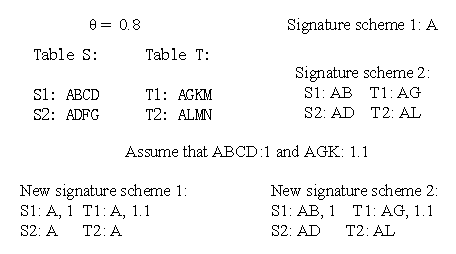
\includegraphics[scale=0.8]{figures/signature_example1}
 \caption{Illustration to the difference of signature schemes}
\label{fig:signature_example1}
\end{figure}

A Count-Min (CM) sketch with parameters ( $\varepsilon, \delta$) is represented by a two-dimensional
array counts with width $w$ and depth $d$. Given parameters ($\varepsilon, \delta$), set
$w$ = $\lceil \frac{e}{\varepsilon} \rceil$ and $d$ = $\lceil ln \frac{1}{\delta} \rceil $. Each entry of the array is initially zero.


When a data item ($w,i$) arrives, meaning that the signature $w$ has the length $i$, then $i$ is added to one cell in each row; the counter is determined by $h_j$. Formally, set $\forall 1 \leq j \leq d$, then count[j,$h_j(i)$]


The space used by Count-Min sketches is the array of $wd$ counts, which takes $wd$ words, and $d$ hash
functions, each of which can be stored using 2 words when using the pairwise functions described in [27].

Estimation procedure. Our estimation for $S \bigodot T $ = $min_j S_j \bigodot T_j $


\begin{theorem}
With a probability 1- $\delta$, The upper bound and lower bound of Composite signature estimation is
 $S \bigodot T $ and  $S \bigodot T $ + $\varepsilon |S| |T|$, respectively.
\end{theorem}

\begin{theorem}
Our composite signature estimation estimates the lower and upper bounds of algorithms by keeping space $O(\frac{1}{\varepsilon} \log \frac{1}{\delta})$ and
\end{theorem}

\subsubsection{Estimation with length filters}

When we use the CountMin sketch to estimate the effectiveness of length filter. It is to

%We  demonstrate that the returned lower and upper bounds are correct, and then we analyze its space and time complexities.
%
%Given a bucket with the sum $S$ and the number of lengths is $n$, the maximal frequency is $Max$, and the minimal frequency is $Min$, Suppose each element can join with other adjacent $\mu$ elements.
%
%Let $t = \frac{S}{M}$. Without the loss of generality, we assume that $t_1 \geq t_2$. Therefore, the upper bound of the join size is:
%
%$t_2 \times \mu M_1 M_2$ + $(t_1-t_2) \times \mu M_1$ = $\mu M_1 S_2$.
%
%In other words:
%
%$max(S_1 \cdot M_2, S_2 \cdot M_1)$
%
%The lower bound of the join size is
%
%$\mu \cdot (S_1+ S_2)$
%
%When we separate the data to two parts, we can try to make them the same for the sum.
%
%\begin{theorem} With at most $O(\log N)$ storage, we can compute the approximation with length filter. Each new data item needs $O(\log N)$ time to be processed.
%\end{theorem}


\subsection{Extensions for flexible query thresholds} \label{subsec:flexible}

In the previous sections, our model assumes that the search threshold is fixed, and only the query can be changed online. However, in practice users might change the threshold at query-time. Therefore, we now move to a more general case, where both the search string and the threshold are flexible at query-time. The new challenge here is that we do not know the threshold in advance and thus we cannot determine the number of signatures of each record. A na\"{i}ve method is to compute the signatures of records in the table online according to the given threshold, which  is clearly prohibitively expensive. Next we build a new index called \textit{FSI-trees} (Flexible Signature Indexing) by extending SI-trees to solve this problem.

Suppose that all meaningful thresholds distribute in the range between 0.99 to 0.50. Then we select some \textit{representative thresholds}, e.g. 0.95, 0.90, etc.   For each representative threshold, we generate signatures for each record. See an example in Figure \ref{fig:FSI}(a). Note that the signatures of a string for lower thresholds are guaranteed to become signatures of that for higher thresholds. To build an FSI-tree,  the length and fence entries of SI-trees remain the same. But each fence entry points to a set of I-lists which come from \textit{all} representative thresholds. Further, each element in the I-list of a signature token $s$ is a binary tuple ($q$, $\theta$), where $q$ is a record ID and $\theta$ is the minimal threshold for which this signature $s$ appears in $q$. For example, in Figure \ref{fig:FSI}(b), the token ``\textsf{Computing}''  is a signature of $q_1$ for all thresholds $\geq 0.5$.

We extend the QP-search algorithm for flexible thresholds. The algorithm almost remains the same, but  the only  change (See Algorithm \ref{algo:QP-flexible}) is that we select the string candidates in I-lists by checking their thresholds (Line 3).

An astute reader may notice that our method possibly introduces more candidates because of the gap between representative thresholds and online thresholds. For example, given a query threshold 0.83, suppose that the closest representative threshold is 0.80. Then  the number of signatures for threshold 0.80  may be greater than that for 0.83. But we argue that the problem  has actually a little impact on the final performance of query processing. To understand this, assume that gap between two representative thresholds is no more than 0.05 (that means, only 11 representative thresholds are ``materialized'' with signatures between 0.99 and 0.50). It can be proved that given a string $s$, the difference between the numbers of signatures for thresholds $\theta_1$ and $\theta_2$ is $\lceil  |\theta_1 - \theta_2|   \cdot |s| \rceil$. Considering a string $|s|$=10, we have 0.05 * 10 =0.5, That is, for most records in the table, the extra number of signatures due to the thresholds gap  is bounded by 0.5. Therefore, as our experimental results show in Section \ref{subsec:searchalgorithms}, the performance of our algorithms for flexible thresholds is comparable to that for static thresholds.





\input{updatingTaxonomy}

\input{extension}

\section{Experimental analysis}

We implemented various algorithms presented in this paper, and experimentally compare their performance for string similarity joins with taxonomies. The experiments study both the effectiveness and efficiency of proposed measures and join algorithms.  


 

\subsection{Experimental setting and datasets}

We  implemented all similarity measurement and algorithms in Java $1.6.0$ and run on a
Windows XP with dual-core Intel Xeon CPU 4.0GHz, 2GB RAM, and a 320GB hard disk.


We use three real datasets and one random dataset: Consensus data (\textbf{Consensus}),
Crimes data  (\textbf{Crime}), and Life science data
(\textbf{Life}) and three taxonomies. These datasets differ from each other in terms of data-size and string-length, taxonomy-size, taxonomy-tree-complexity, . Our goal in choosing these diverse sources is to understand the usefulness of algorithms in different real world environments.


\smallskip
%\noindent \textbf{{Consensus data}}: Extraction was done by Barry Becker from the 1994 Census database. native-country: Include 32561 instances, we can perform the similarity joins on multiple column, including countries, occupation, marital-status, education and workclass. The feature of this dataset is to perform the similarity join against multiple columns.

\noindent \textbf{{Crime data}}: This dataset reflects reported incidents of crime that occurred in the City of Chicago from 2001 to present \footnote{https://catalog.data.gov/dataset/crimes-2001-to-present-398a4}. The dataset contains more than 65,000 records/rows of data and cannot be viewed in full in Microsoft Excel.


\noindent \textbf{{Library data}}: This dataset\footnote{http://www.theeuropeanlibrary.org/tel4/access/data/opendata/details}  constitutes the subset of The European Library's aggregated data that is made openly available by its partner libraries. 




\noindent \textbf{{Life science data}}: As a subject matter taxonomy for our expert matching
in this medicine domain, we used the Medical Subject Head-
ings (MeSH)\footnote{https://www.nlm.nih.gov/mesh} that is a biomedical controlled vocabulary
consisting of 26k+ biomedical terms arranged in a taxonomic
structure introduced by National Library of Medicine
(NLM). The benefits of using MeSH terms have been increasingly
highlighted in various applications for biomedical
concept and knowledge extraction from text [11]. We obtained one million gene/protein records
from the Expasy website ({\footnotesize http://www.expasy.ch/sprot}).
Each record contains an identifier (ID) and its name. In this dataset, each ID has $5\sim22$ synonyms. We generated 10,000 synonym rules describing gene/protein
equivalent expressions.

\noindent \textbf{{Synthetic data}}: We generate data by random creating a taxonomy tree with varied tree fanout and tree depth. 

\begin{table}[t]
\centering
\begin{tabular}{|@{\hspace{1mm}}c@{\hspace{1mm}}|@{\hspace{1mm}}c@{\hspace{1mm}}|@{\hspace{1mm}}c@{\hspace{1mm}}|@{\hspace{1mm}}c@{\hspace{1mm}}|}
%{|p{1cm}|p{1cm}|p{1cm}|p{1cm}|p{1cm}|p{1cm}|p{1cm}|}
%|c|m{6cm}|
\hline
 \textbf{Name} & \textbf{\# of nodes} &  \textbf{Depth} & \textbf{Fan-out} \\
  \hline \hline

  Wikipedia & 10,000 & 5 & 2,000 \\

   MeSH category  & 56326 & 5 &  18/3.4 \\

  WordNet & 10,000  & 5 & 2,000  \\

  \hline
\end{tabular}
\caption{Characteristics of taxonomy datasets.}
\label{tab:data}
\end{table}

\begin{table}[t]
	\centering
	\begin{tabular}{|@{\hspace{1mm}}c@{\hspace{1mm}}|@{\hspace{1mm}}c@{\hspace{1mm}}|@{\hspace{1mm}}c@{\hspace{1mm}}|@{\hspace{1mm}}c@{\hspace{1mm}}|}
		%{|p{1cm}|p{1cm}|p{1cm}|p{1cm}|p{1cm}|p{1cm}|p{1cm}|}
		%|c|m{6cm}|
		\hline
		\textbf{Name} & \textbf{\# of records} &  \textbf{Length} & \textbf{\# of T-node per string} \\
		\hline \hline
		
		Crime records & 10,000 & 5 & 2,000 \\
		
		MeSH terms  & 935249 & 2.1 &  1.5/9 \\
		
	    Library records & 36,000  & 5 & 2,000  \\
		
		\hline
	\end{tabular}
	\caption{Characteristics of join datasets.}
	\label{tab:data}
\end{table}


%\begin{figure}
%  \small
%  \centering
%  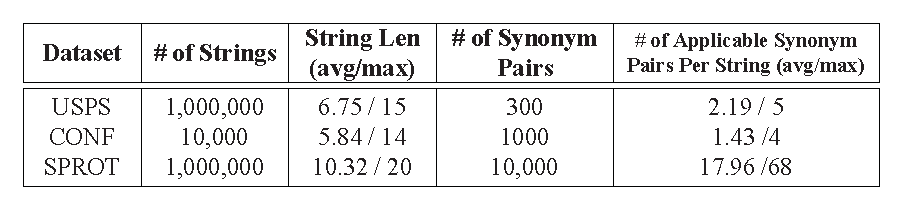
\includegraphics[width=\linewidth]{figures/Characteristics_Datasets}
%   \vspace{-6mm}
%  \caption{Characteristics of Datasets.}
%  \label{tab:data_characteristics}
%\end{figure}


Figure~\ref{tab:data_characteristics} gives the characteristics of the
three datasets.

\subsection{Effectiveness of taxonomy for string joins}

The first experiment is to demonstrate the effectiveness of
taxonomy for string joins. We compared our
two measures: Jaccard similarity, full expansion
  (\textbf{Full}), and  our similarity with taxonomy.

For each of the three datasets, we performed the experiments by conducting a similarity join between the
query table $T_Q$ and the target table $T_T$ as follows: (1) $T_Q$ consists of 100 manually selected
full names, and (2) $T_T$ has 500 records where 100 of them
are the correct abbreviations of the corresponding records in $T_Q$
(i.e., the ground truth), and the other 400 random records are selected from string collections. This is to
ensure that there is only one correct matching record in $T_T$ for each
 record in $T_Q$.

Quality of Measures.

In Figure \ref{fig:quality}, we report the quality of the measures by testing the \textit{Precision} (short for ``P''),  \textit{Recall} (``R''), and \textit{F-measure$=\frac{2\times P \times R}{P+R}$} (``F'') on three datasets. We observe that:

\noindent$\bullet$ The similarity measures using synonyms (including \textit{JaccT}, \textit{Full} and \textit{SE}) obtain higher scores than Jaccard which does not consider synonym pairs. The reason is that without using synonyms, Jaccard has no chance to improve the similarity.

%\noindent$\bullet$  \textit{Full} achieves a comparable performance with \textit{JaccT}. Note that \textit{JaccT}  selects only appropriate synonyms to increase the similarity, but \textit{Full} utilizes all the applicable rules and most rules in \textit{Full} is useful, since it is not common that synonyms contain ambiguous meanings. In addition, note hat \textit{Full} is much more efficient than \textit{JaccT}, which will be demonstrated later.


\noindent$\bullet$ \textit{SE} significantly outperforms \textit{JaccT} in each dataset. For example, on SPROT dataset, the F-measures of \textit{SE} and \textit{JaccT} are $0.82$ and $0.52$, respectively. The main reason is that: an abbreviation may have various full expressions and the join records may contain the combination of multiple expressions. Therefore \textit{SE} can apply multiple rules, while \textit{JaccT} can apply only one. Note that such situation is not rare in the real world, as one fragment of a string likely involves multiple synonym rules. We illustrate one example on each of three datasets in Figure \ref{fig:quality} to compare the performance of four similarity measures. For example, see CONF data in Figure \ref{fig:quality}, ``\textsf{VLDB}'' has two different full expressions, i.e., ``\textsf{International Conference on Very Large Databases}'' ($r_1$) and ``\textsf{Proceedings of the VLDB Endowment}''($r_2$), and $s1$ contains these two expressions.  \textit{SE} applies both $r_1$ and $r_2$ to $s_2$ to obtain a high similarity score, i.e., 0.93, while \textit{JaccT} can only apply $r_2$ to $s_2$ and the similarity is only $0.57$. Assume that the join threshold is 0.8, then  \textit{JaccT} can not find the correct answer while \textit{SE} can.


\begin{figure*}[h]
	\small
	\centering
	\includegraphics[width=\linewidth]{figures/measure01}
	\caption{Quality of similarity measures (P: precision, R: recall, F: F-measure) and examples to illustrate the quality of similarity measures. }
	\label{fig:quality}
\end{figure*}

\begin{figure}[t]
	\centering
	\includegraphics[scale=0.25]{figures/TrieJoin}
	\caption{Three join algorithms}
	\label{fig:similaritygeaph}
\end{figure}

\begin{figure}
	\centering
	\includegraphics[scale=0.25]{figures/LCPTimes}
	\caption{LCP times for two algorithms}
	\label{fig:LCPTimes}
\end{figure}

\begin{figure}
	\centering
	\includegraphics[scale=0.25]{figures/selectratio}
	\caption{Three algorithms with varied selectivity ratios (5M records, random data)}
	\label{fig:selectratio}
\end{figure}

\subsection{Efficiency and scalability of exact-join algorithms}

The second set of experiments is to test the efficiency and scalability of
various exact-joins algorithms. We compared our algorithms, the \textbf{baseline}
and \textbf{TIndex}.

Metrics.

 We took the following measures: (i) the running time (including filtering time, verification time and the time for building QP-tree for a query), and (ii) the size of candidates.

Running Time and Scalability.
Figure~\ref{fig:search_scalability_datasize} shows the running time of the four search algorithms, where the threshold is $0.9$. As shown, the running times of Search-baseline(F) and Search-baseline(S) have an exponential growth, whereas QP-search(F) and QP-search(S) scale better (i.e., linear). The reason is that QP-search generates less candidates for the final verification.

To study the scalability of algorithms with the various threshold values, we plotted Figure \ref{fig:search_scalability_threshold}. As shown, the running time of the algorithms decreases with the growth of the threshold values. In addition,  QP-search scales well with various thresholds. In contrast, when the threshold value is small, the running time of Search-baseline increases significantly. For example, in Figure \ref{fig:search_scalability_threshold}(b), when threshold=0.9, the running time of Search-baseline is about 7 times more than that of QP-search. In addition, when the threshold=0.5, the performance of QP-search is at least 15 times better than Search-baseline.

We then study the time cost of Search-baseline and QP-search with different number of synonyms. Recall that the similarity search proceeds to  generate signatures (or QP-index) for a given query, and then to filter the candidates by checking the overlaps of the signatures, and finally to verify the similarity. Therefore, we reported the individual execution time of signature-generation, filtering and verification in Figure  \ref{fig:search_synonyms_conf}. As seen from this figure, we observe that QP-Search(S) significantly outperforms Search-baseline(S) by one order of magnitude. The main reasons are as follows:



(i)  Search-baseline(S) needs to union all the signatures computed from each possible expanded set, while QP-Search(S) directly utilizes the intermediate signatures. Therefore, the time of signature-generation of QP-Search(S) is less than that of Search-baseline(S).

(ii) For the filtering phase, QP-Search(S) utilizes the SI-Index and QP-index to achieve stronger filtering power than Search-baseline(S). Thus, the filtering time of QP-Search(S) is less than Search-baseline(S). In addition, due to the powerful filtering, QP-Search(S) generates less candidates than that of Search-baseline(S). For example, in Figure  \ref{fig:search_synonyms_conf}, we reported the number of candidates for each query. As shown, the number of candidates of Search-baseline(S) is about one order of magnitude more than that of QP-search(S).

(iii)  QP-Search(S) spends less time on verifying the candidates than Search-baseline(S). Therefore, the verification time of QP-Search(S) is less than that of Search-baseline(S).

Therefore, QP-Search(S) outperforms Search-baseline(S) in each of the three phases.  Experiments in USPS and SPROT datasets have the similar trend (as shown in Figure \ref{fig:search_synonyms_usps} and Figure \ref{fig:search_synonyms_sprot}, respectively).

\subsection{Efficiency and scalability of approximate-join algorithms}

The third set of experiments is to test the efficiency and scalability of
approximate-join algorithms. We compared the algorithms \textbf{baseline}
and \textbf{SI-Join}.  We implemented all algorithms using both
prefix and LSH filters. Therefore, with respect to the algorithms using
LSH scheme, we append ``-LSH'' to the name, e.g., JaccT-LSH denotes the
JaccT algorithm using LSH scheme. Note that, we use the false negative
ratio $\delta \leq 5\%$, i.e., the accuracy is $1-\delta \geq 95\%$. The
parameters $k$ and $l$ should satisfy: $\delta \geq
(1-\theta^k)^l$~\cite{journals/tods/XiaoWLYW11}. For example, if
threshold $\theta=0.8$, $k=3$, then $l$ should be at least $5$ to
guarantee $> 95\%$ accuracy.

Metrics. We took the following measures: (i) the size of signatures, (ii) the filtering ratio of the algorithms, which is typically defined as the number~of~pruned~string~pairs divided by the total number of string pairs; and (iii) the running time (including filtering time and verification time).

Number of Signatures.


We first performed experiments to report the number of signatures of a
query string. It has a major impact on the query time, as both \textit{JaccT} and
our join algorithms need to frequently check the overlaps of string
signatures. The results are reported in Figure~\ref{fig:signature-size}.
For both prefix and LSH schemes, the number of signatures of our
expansion-based algorithms is smaller than that of \textit{JaccT}. The reason is
that based on a transformation framework, \textit{JaccT} is more likely to
include new tokens into signatures than ours. In addition, we observe
that the size of signatures in the LSH scheme is greater than that in
prefix scheme, and the gap increases when the threshold decreases. As we
will see shortly, this results in substantial overhead of filtering time
for the LSH scheme.


\textbf{Filtering Power.}

We investigated the filtering power of different algorithms in
Figures~\ref{fig:filter_ratio_prefix} and \ref{fig:filter_ratio_LSH} using
prefix and LSH schemes, respectively. The experiments were performed on
USPS and SPROT datasets for self-join. For prefix-based algorithms,
Join-baseline is slightly better than JaccT, while SI-Join has a substantial
lead over JaccT and Join-baseline. These results are mainly because of the
additional filtering power in SI-Join brought by length filtering and
signature filtering. Next, for LSH-based algorithms, Figure
\ref{fig:filter_ratio_LSH} demonstrates the similar trend. That is,
SI-Join is the winner in all settings by varying the parameters $k$ and
$l$. Compared to the prefix scheme, LSH has a slightly higher filtering
ratio when parameters are set optimally (e.g. 99.2\% v.s. 98.9\% in USPS
data, with threshold 0.9). On the other hand, note that LSH may filter
away correct answers, resulting in false negatives, as can be seen from
the false negative percentages shown in
Figure~\ref{fig:filter_ratio_LSH}.

\textbf{Effects of different filters.}

We analyzed the effects of different filters, i.e., signature-filters, length-filters and  signature-plus-length. As shown in Figure \ref{fig:filter_methods},  signature-plus-length filters obtain the strongest filtering power on all the datasets, which explains why our algorithms use these two kinds of filters together. There is no absolute winner between signature filters and length filters. In particular, signature filters have stronger filtering power on the USPS dataset (Figure \ref{fig:filter_methods}(a)), while the opposite situation occurs in the SPROT dataset (Figure \ref{fig:filter_methods}(c)), i.e., length filters beat signature filters. On the CONF dataset (Figure \ref{fig:filter_methods}(b)), when the threshold value is small, signature filters win length filters. However, when the threshold value is high, length filters beat signature filters. Therefore, the individual effects of signature filters and length filters depend on the data sets and the thresholds, and the combined structure of both (i.e. SI-tree) achieves the best results.



\begin{figure}[t]
	\centering
	\includegraphics[scale=0.25]{figures/Drawing1}
	\caption{Nested loop and SS filter}
	\label{fig:similaritygeaph}
\end{figure}


\textbf{Running Time and Scalability.}


Figure~\ref{fig:scalability} and Figure \ref{fig:scalability_LSH} show the running time of five join algorithms based on prefix and LSH schemes, respectively, where the join threshold is $0.8$. The x-axis represents the join data size. As shown, the running times of both JaccT and Join-baseline (i.e., Join-baseline(F), Join-baseline(S)) have an exponential growth, whereas SI-Join (i.e., SI-Join(F), SI-Join(S))  scales better (i.e., linear) than Join-baseline and JaccT. The reason is that SI-Join methods have more efficient filtering strategies and generate smaller size of candidates.  In addition, in order to study the scalability of algorithms with the increase of the number of rules, we plot Figure \ref{fig:synonyms}(b), where  SI-Join(F) (i.e., SI-Join with the full-expansion) is a clear winner in algorithms using rules: it is insensitive to the number of rules and thus able
to outperform other methods when one string involves more than 10 rules.


\smallskip

\subsection{Estimation-based filter selection}

The following tables shows the results for our estimation and the optimal filters by trying all possibilities. This is the join operations for all 1K data self-joins.

By varying the thresholds:

Thresholds: 0.75, Optimal 19.25K candidate, estimation: 19.30K

Thresholds: 0.8, Optimal 19.8K candidate, estimation: 19.9K

Thresholds: 0.85, Optimal 20.1K candidate, estimation: 20.8K

Thresholds: 0.9, Optimal 16.7K candidate, estimation: 18.4K

Thresholds: 0.95, Optimal 18.8K candidate, estimation: 19.05K

\noindent \textbf{Summary} ~~ Finally, we summarize the main findings.

(1) Considering four similarity measures, we observe that \textit{Jaccard} is inadequate due to its complete neglect of synonym rules. \textit{JaccT} is not efficient because it enumerates all transformed strings and entails large query overhead. \textit{Full-expansion} is extremely efficient, but its F-measure is not as good as \textit{Selective-expansion}, which makes a good balance between effectiveness and efficiency.

(2)	With respect to the similarity searches and joins,  QP-search and SI-join are the winners in the settings, respectively over the previous algorithms (i.e., \textit{JaccT}) and baseline methods. Note that we achieve a speedup of up to 50$\sim$300x on three data sets over the state-of-the-art approach.

(3) Finally, 2DHS synopsis offers very good results, and is extremely efficient to estimate the filtering power of different filters, ( $<$ 1 second ,  accounting for only 1\% of the total running time),  which strongly motivates its application in practice.



\section{Related work} \label{sec:relatedwork}

Taxonomy is the practice and science of classification. Many taxonomies have a hierarchical structure, but this is not a requirement. In this work, we study to leverage the existing taxonomy to improve the accuracy of string record join in databases. Such a taxonomy could be constructed manually
through experts and community efforts, as in WordNet
[4], Cyc [14], and Freebase. With the advantage of freshness
and informativeness, automatic taxonomy construction has
been extensively studied recently, for example, in [20, 22,
18, 21, 26]. WikiTaxonomy [18] and YAGO [22] may be the
most notable efforts, which attempt to derive a taxonomy
from Wikipedia categories. With more web data, Probase
[26] aims at building a unified taxonomy of worldly facts.

In recent years, we have witnessed the emergence of various efforts to enhance the effectiveness of string similarity joins by using synonyms \cite{conf/sigmod/LuLWLW13,conf/icde/ArasuCK08,conf/cpm/BarbayGMR06,conf/vldb/ArvindSR09}.
The traditional similarity functions consider only syntactic similarities, e.g., number of common
words or $q$-grams. But there are many important cases where syntactically different
strings can represent the same real-world object. For example,
``\textsf{Bill}'' is a short form of ``\textsf{William}'', and ``\textsf{ICDE}'' is an abbreviation of  ``\textsf{International Conference on Data Engineering}''.  Given two collections of strings,  synonym-based similarity functions can utilize the available synonyms to find string pairs which are semantically similar. While those methods improve the effectiveness of string joins, a synonym dictionary does not contain information such as
``\textsf{Helsinki is the capital of Finland}'', or `\textsf{`Apple 6 Plus is a new model of iPhone}''. Still, term pairs such as ``\textsf{Helsinki}'' and ``\textsf{Finland}'', ``\textsf{Apple 6 Plus}'' and ``\textsf{iPhone}''  have strong semantic correlations.



Taxonomies are is-a hierarchies of concepts, topics, or keywords. Since they represent ontology specializations, they may be
used to provide meaningful knowledge representations and, thus, support users in understanding the semantic meaning of a
resource and the related domain.
Several efforts to integrate taxonomies in the Data mining and Knowledge Discovery (KDD) process have been done. For
instance, taxonomies have already been exploited to (i) discover high level correlations among data [9�C13], (ii) perform textual
data analysis and summarization [14,15,35,36], (iii) improve user browsing by looking into the results of Web search engines
[37], and (iv) enhance the quality of recommendation systems [17,38]. This paper focuses on exploiting taxonomy information to
enrich data used for classification. To the best of our knowledge, it is the first attempt to integrate high level and multi-faceted
knowledge into classifier construction.


Several types of Similarity Join have been proposed in the
literature, e.g., distance range join (retrieves all pairs whose distances
are smaller than a predefined threshold $\varepsilon$) [2, 3, 4, 5, 6,
7], k-Distance join (retrieves the k most-similar pairs) [8], and
kNN-join (retrieves, for each tuple in one table, the k nearest neighbors
in another table) [9, 10, 11]. The distance range join
has been one of the most studied and useful types of Similarity
Join. This type of join is commonly referred to simply as Similarity
Join and is the focus of this paper. Among its most relevant
implementation techniques, we find approaches that rely
on the use of pre-built indices, e.g., eD-index [3], D-index [4],
and List of Twin Clusters (LTC) [12]. These techniques strive
to partition the data while clustering together the similar objects.
While these indexing techniques support the SJ operation
they also have some shortcomings: D-index and eD-index may
require rebuilding the index to support queries with different $\varepsilon$,

Approximate string matching includes finding (sub)strings
that resemble a given query string. It is a well-researched
topic and has many applications, such as data cleansing [1],
spelling correction [19], query autocompletion [33], near duplicate
detection [25, 32], approximate named entity recognition
[29], and bioinformatics [20, 27, 35].
Due to the sheer amount of literature in this area, we will
focus on most related recent results and refer readers to the
excellent surveys [13, 22] and tutorials [3, 12, 16] for a comprehensive
treatment of the topic.
Based on the types of the queries, recent work focuses either
on efficient single query processing (typically named string
similarity queries) [1, 6, 9, 11, 18, 25, 28, 31], or the similarity
join which can be treated as processing a batch of similarity
queries [2, 8, 10, 12, 14, 17, 28, 29, 34, 35]. Most recently,
Jiang et al. [15] experimentally evaluate and analyze many of
the existing similarity join algorithms.


$\mathbf{Prefix filter.}$ Since the prefix
filter is effective, many methods are proposed to optimize it
for different similarity operators [6,16,20,24,26,28,29]. ED-
join [12,28] proposed a location-based mismatch filter to re-
duce prefix length and a content-based mismatch filter to
reduce the number of candidates for ED. Pivotal prefix filter [4] reduced the prex length for ED. PassJoin [17] pro-
posed segment filter to improve pruning power. PPJoin [29]
used the positions of prefix and suffix to improve pruning
power for token-based similarities. Length filter was pro-
posed to prune dissimilar answers based on length difference [8]. TrieJoin [23] used a different framework that directly computed real similarity using the trie structure.





\section{Conclusion}

In this paper, we presented a framework which use the exsting taxonomy to perform exact and approximate.
concepts included.

We introduce a new query type, approximate string join, with taxonomy. We propose processing
models for taxonomy queries, and introduce how to build
an additional index (besides the inverted index) to support
efficient query processing. In particular, we study the problem
of how to optimize this additional index based on a
workload of queries, with the goal of minimizing query processing
cost, and propose algorithms with performance guarantees.
Our index optimization techniques are tested using
real datasets and are shown to be effective and robust.


\bibliographystyle{abbrv}
\bibliography{localrefs}



\end{document}
